实际参照平台为Quanser公司的2 DOF Planar Robot绘图实验机器人，如图\ref{fig:real_robot}所示。制造商介绍与用户手册表明，该设备采用五杆并联机构，两台带减速器的电机驱动基座关节，公共末端安装笔，并由电磁机构完成落笔，以纸上轨迹展示机器人运动效果\cite{barnard2009,quanser2013}。因此，轮廓描绘不仅是抽象的点轨迹，也对应真实设备中的笔尖定位任务。

\begin{figure}[htbp]
\centering
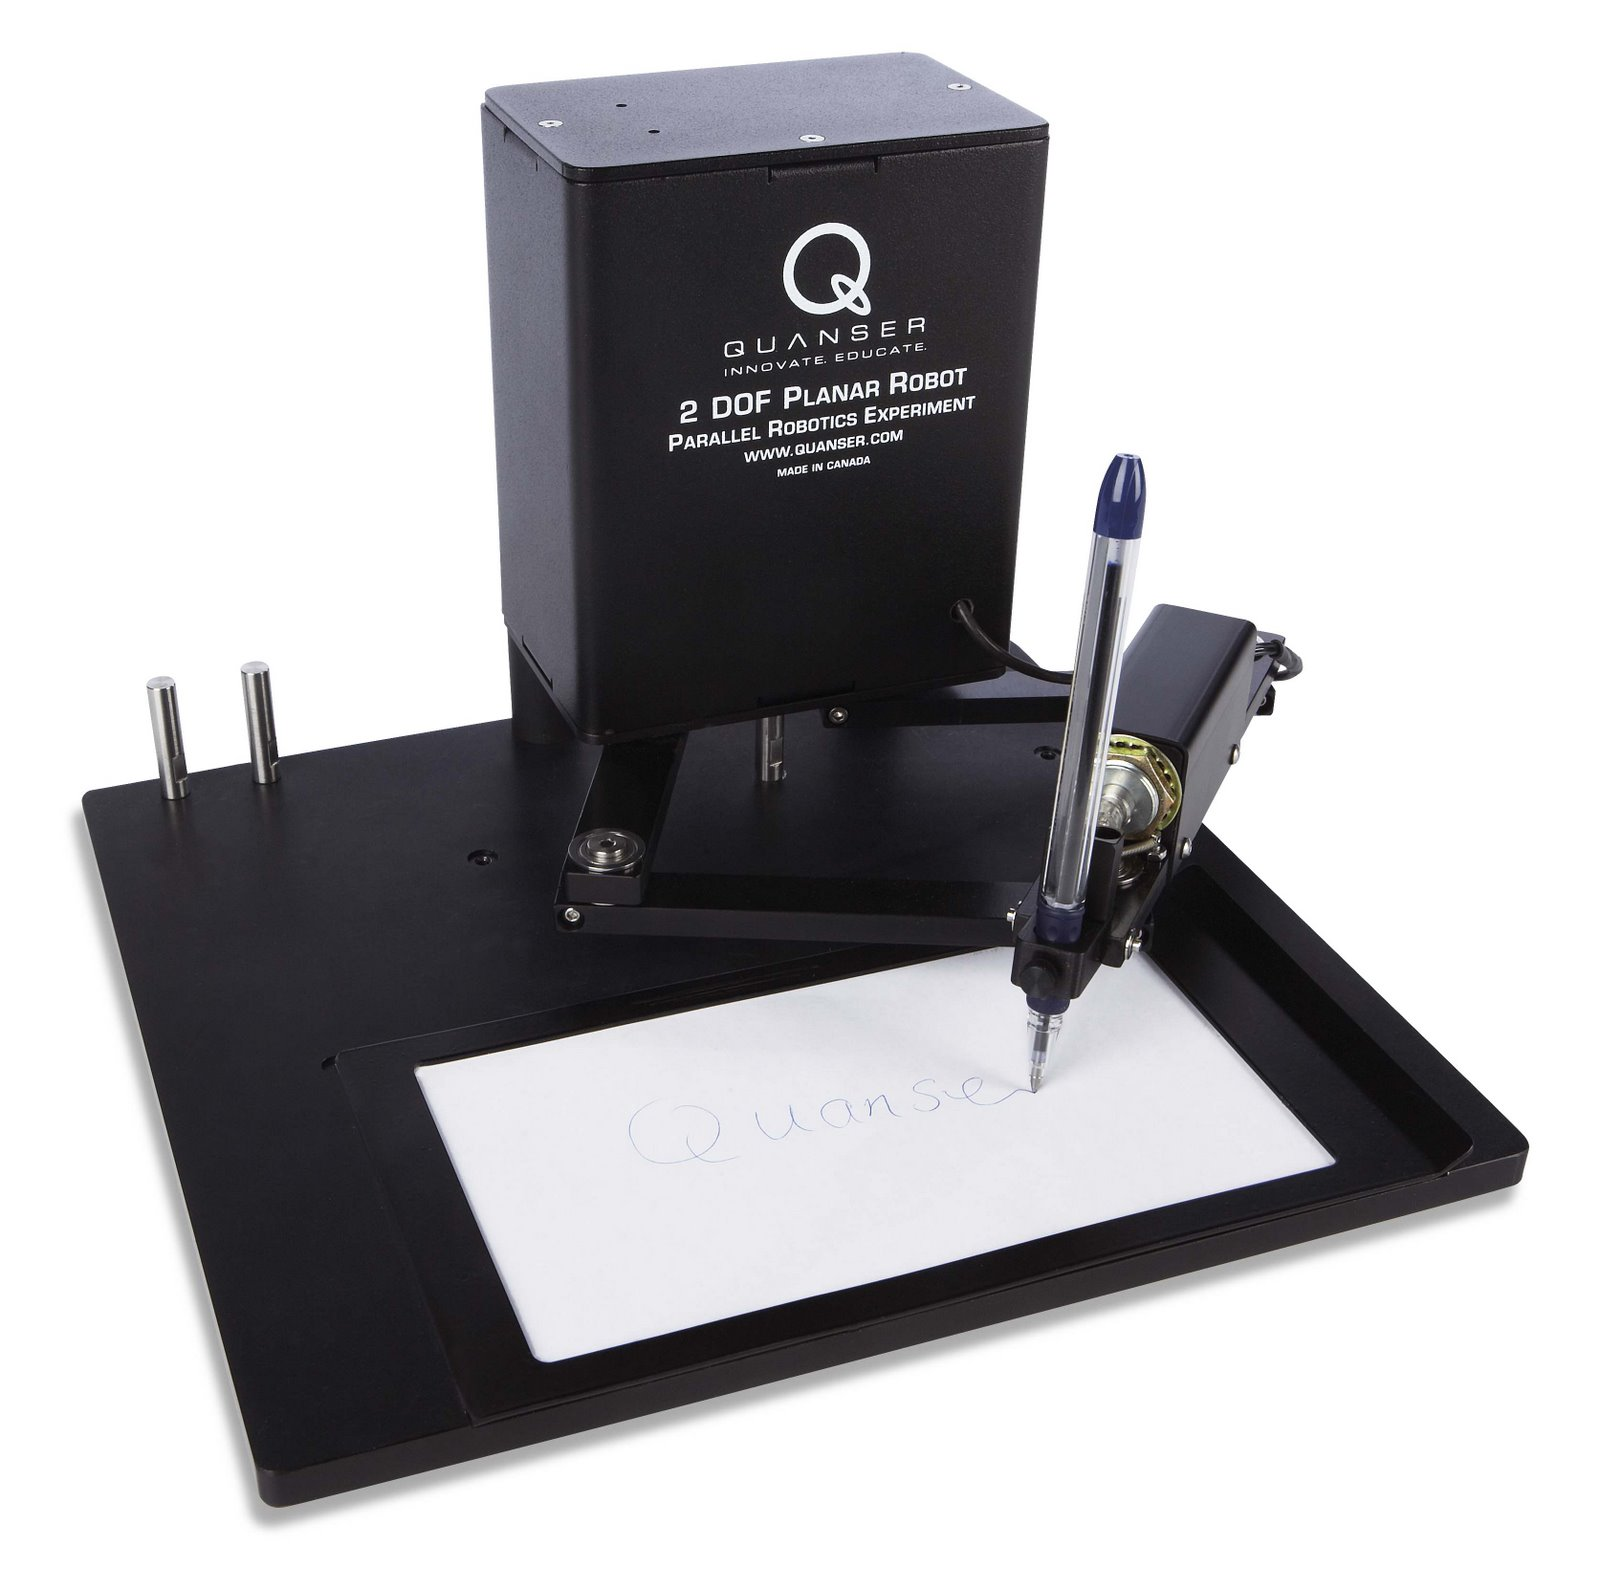
\includegraphics[width=0.66\linewidth]{Quanser_2009_2DOF_Planar_Robot_official_blog.jpg}
\caption{Quanser 2 DOF Planar Robot实物及笔式绘迹配置。来源：制造商官方工程博客，Barnard，2009\cite{barnard2009}；\textcopyright\ Quanser，原图未修改，作为实际机构与应用场景的引用图片。}
\label{fig:real_robot}
\end{figure}

本文保留该平台的五杆拓扑与笔式绘迹需求，进一步设定一个竖直工件板上的椭圆轮廓标记场景：工具在宽$80\units{mm}$、高$50\units{mm}$的轮廓上运动，并在$4\units s$内从静止出发、闭合后回到静止。与桌面绘图相比，竖直安装使杆件和工具的重力直接参与板面内负载，适合分析拉格朗日和牛顿—欧拉方程中的重力项。表\ref{tab:parameters}所列尺寸、质量及安装方向均为本报告的课程设计输入，未将其标作Quanser原机规格，也不将数值仿真表述为原机实测或参数复现。

在工程实施中，完整描绘流程还包括定位板面、抬笔到起点、落笔、沿轮廓运动与抬笔退出。本文研究其中落笔后的二维轮廓段；法向落笔行程作为独立动作，不引入二维模型的自由度。安装方向的影响将在第3节用同一机构从水平到竖直的倾角扫描进行定量说明。
